\documentclass[12pt,a4paper]{article}

%\usepackage[left=1.5cm,right=1.5cm,top=1cm,bottom=2cm]{geometry}
\usepackage[in, plain]{fullpage}
\usepackage{array}
\usepackage{../../../pas-math}
\usepackage{../../../moncours}


%\usepackage{pas-cours}
%-------------------------------------------------------------------------------
%          -Packages nécessaires pour écrire en Français et en UTF8-
%-------------------------------------------------------------------------------
\usepackage[utf8]{inputenc}
\usepackage[frenchb]{babel}
\usepackage[T1]{fontenc}
\usepackage{lmodern}
\usepackage{textcomp}



%-------------------------------------------------------------------------------

%-------------------------------------------------------------------------------
%                          -Outils de mise en forme-
%-------------------------------------------------------------------------------
\usepackage{hyperref}
\hypersetup{pdfstartview=XYZ}
%\usepackage{enumerate}
\usepackage{graphicx}
\usepackage{multicol}
\usepackage{tabularx}
\usepackage{multirow}


\usepackage{anysize} %%pour pouvoir mettre les marges qu'on veut
%\marginsize{2.5cm}{2.5cm}{2.5cm}{2.5cm}

\usepackage{indentfirst} %%pour que les premier paragraphes soient aussi indentés
\usepackage{verbatim}
\usepackage{enumitem}
\usepackage[usenames,dvipsnames,svgnames,table]{xcolor}

\usepackage{variations}

%-------------------------------------------------------------------------------


%-------------------------------------------------------------------------------
%                  -Nécessaires pour écrire des mathématiques-
%-------------------------------------------------------------------------------
\usepackage{amsfonts}
\usepackage{amssymb}
\usepackage{amsmath}
\usepackage{amsthm}
\usepackage{tikz}
\usepackage{xlop}
%-------------------------------------------------------------------------------



%-------------------------------------------------------------------------------


%-------------------------------------------------------------------------------
%                    - Mise en forme avancée
%-------------------------------------------------------------------------------

\usepackage{ifthen}
\usepackage{ifmtarg}


\newcommand{\ifTrue}[2]{\ifthenelse{\equal{#1}{true}}{#2}{$\qquad \qquad$}}

%-------------------------------------------------------------------------------

%-------------------------------------------------------------------------------
%                     -Mise en forme d'exercices-
%-------------------------------------------------------------------------------
%\newtheoremstyle{exostyle}
%{\topsep}% espace avant
%{\topsep}% espace apres
%{}% Police utilisee par le style de thm
%{}% Indentation (vide = aucune, \parindent = indentation paragraphe)
%{\bfseries}% Police du titre de thm
%{.}% Signe de ponctuation apres le titre du thm
%{ }% Espace apres le titre du thm (\newline = linebreak)
%{\thmname{#1}\thmnumber{ #2}\thmnote{. \normalfont{\textit{#3}}}}% composants du titre du thm : \thmname = nom du thm, \thmnumber = numéro du thm, \thmnote = sous-titre du thm

%\theoremstyle{exostyle}
%\newtheorem{exercice}{Exercice}
%
%\newenvironment{questions}{
%\begin{enumerate}[\hspace{12pt}\bfseries\itshape a.]}{\end{enumerate}
%} %mettre un 1 à la place du a si on veut des numéros au lieu de lettres pour les questions 
%-------------------------------------------------------------------------------

%-------------------------------------------------------------------------------
%                    - Mise en forme de tableaux -
%-------------------------------------------------------------------------------

\renewcommand{\arraystretch}{1.7}

\setlength{\tabcolsep}{1.2cm}

%-------------------------------------------------------------------------------



%-------------------------------------------------------------------------------
%                    - Racourcis d'écriture -
%-------------------------------------------------------------------------------

% Angles orientés (couples de vecteurs)
\newcommand{\aopp}[2]{(\vec{#1}, \vec{#2})} %Les deuc vecteurs sont positifs
\newcommand{\aopn}[2]{(\vec{#1}, -\vec{#2})} %Le second vecteur est négatif
\newcommand{\aonp}[2]{(-\vec{#1}, \vec{#2})} %Le premier vecteur est négatif
\newcommand{\aonn}[2]{(-\vec{#1}, -\vec{#2})} %Les deux vecteurs sont négatifs

%Ensembles mathématiques
\newcommand{\naturels}{\mathbb{N}} %Nombres naturels
\newcommand{\relatifs}{\mathbb{Z}} %Nombres relatifs
\newcommand{\rationnels}{\mathbb{Q}} %Nombres rationnels
\newcommand{\reels}{\mathbb{R}} %Nombres réels
\newcommand{\complexes}{\mathbb{C}} %Nombres complexes


%Intégration des parenthèses aux cosinus
\newcommand{\cosP}[1]{\cos\left(#1\right)}
\newcommand{\sinP}[1]{\sin\left(#1\right)}


%Probas stats
\newcommand{\stat}{statistique}
\newcommand{\stats}{statistiques}
%-------------------------------------------------------------------------------

%-------------------------------------------------------------------------------
%                    - Mise en page -
%-------------------------------------------------------------------------------

\newcommand{\twoCol}[1]{\begin{multicols}{2}#1\end{multicols}}


\setenumerate[1]{font=\bfseries,label=\textit{\alph*})}
\setenumerate[2]{font=\bfseries,label=\arabic*)}


%-------------------------------------------------------------------------------
%                    - Elements cours -
%-------------------------------------------------------------------------------




\date{}
\title{}


\begin{document}
%\maketitle
\chap[num=2, color=red]{Statistiques à deux variables}{Olivier FINOT, \today }

\section{Série statistique double}

\begin{mydefs}
	\begin{itemize}
		\item Lorsqu'on étudie \kw{deux caractères statistiques} sur une même population, on obtient une \kw{série statistique double}.
		
		\item La représentation d'une série statistique double dans un repère orthogonal forme un \kw{nuage de points}.
		
		\item Le \kw{point moyen} $G$ d'un  nuage de points a pour coordonnées \kw{$(\bar{x}; \bar{y})$}.
	\end{itemize}
	
\end{mydefs}

\begin{myexs}
	\begin{enumerate}
		\item 	Soit ($u_n$) la suite arithmétique de terme initial $u_0 = 1,5$ et de raison $r = -7$.
		
		Le terme de rang $n$ est $u_n = 1,5 + n \times (-7)$ c'est à dire $u_n=1,5 - 7n$.
		
		On a ainsi : 
		\begin{itemize}
			\item $u_4 = 1,5 - 7 \times 4 = -26,5$
			\item $u_{100} = 1,5 - 7 \times 100 = -698,5$
		\end{itemize}
		
		\item Soit ($u_n$) la suite arithmétique de terme initial $u_1 = 14$ et de raison $r = 1,3$.
		
		Le terme de rang $n$ est $u_n = 14 + (n-1) \times 1,3$; c'est à dire $u_n = 12,7 + 1,3n$.

		On a ainsi : 
		\begin{itemize}
			\item $u_4 = 12,7 + 1,3 \times 4 = 17,9$;
			\item $u_{100} = 12,7 + 1,3 \times 100 = 142,7$.
		\end{itemize}
	\end{enumerate}

	
	
\end{myexs}

\newpage

\section{Ajustement affine d'une série statistique et prévisions}


\subsection{Ajustement affine}
\begin{mydefs}
	\begin{itemize}
		\item Si le nuage de points a une forme <<allongée>>, on peut calculer un \kw{ajustement affine} du nuage. 
		\item On obtient ainsi une \kw{droite d'ajustement} (ou droite de régression) qui passe par le point moyen $G$ et au plus près des autres points du nuage.		
	\end{itemize}
\end{mydefs}

\begin{mymeth}
	La droite d'ajustement est obtenue à l'aide du tableur ou de la calculatrice.
\end{mymeth}

\begin{myex}
	La droite d'ajustement obtenue grâce au tableur passe par le point moyen $G$ dont nous avons calculé les coordonnées.
	\begin{center}
		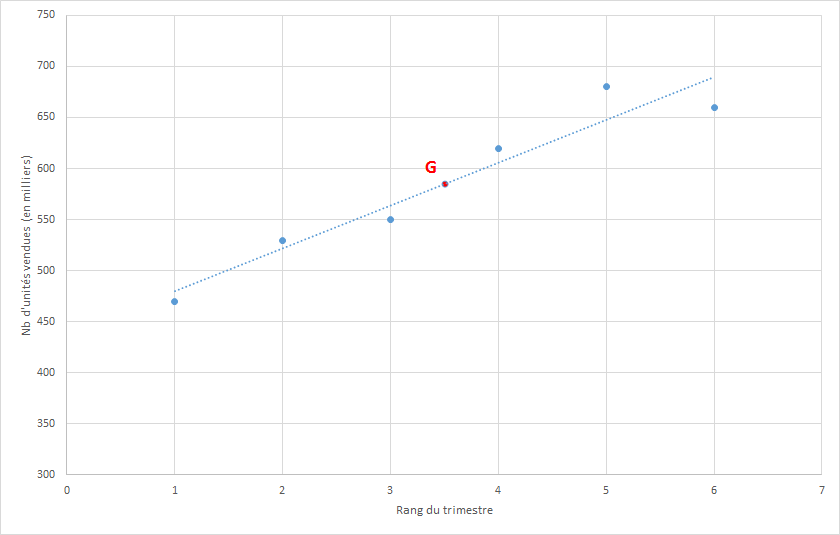
\includegraphics[scale =0.7]{./img/graph2}		
	\end{center}

\end{myex}


\subsection{Prévisions}

\begin{myprop}
	L'équation de type $y = ax +b $ de la droite d'ajustement donne la <<tendance>> de l'évolution de la grandeur $y$ en fonction de celle de $x$. Cette équation permet de réaliser des estimations en supposant que la tendance observée se poursuive.
\end{myprop}

\begin{myex}
	Ici on considère la répartition des prix du gazole dans l'ensemble des 25 stations du département :
	
	\begin{center}
		\begin{tabular}{|@{\ }l@{\ } | @{\ }c@{\ } | @{\ }c@{\ } | @{\ }c@{\ } |@{\ }c@{\ } |@{\ }c@{\ } |@{\ }c@{\ }|@{\ }c@{\ }|@{\ }c@{\ }|@{\ }c@{\ }|@{\ }c@{\ }|}
			\hline
			Prix & 1,368 & 1,369 & 1,374 & 1,375 & \kw{1,377} & \kw{1,379} & 1,385 & 1,408 & 1,450 & 1,460 \\ \hline			
			Nb. de stations & 2 & 5 & 2 & 4 & 1 & 4 & 2 & 1 & 3 & 1 \\ \hline
		\end{tabular}
	\end{center}
	
	\kw{Moyenne} des prix des 25 stations : 
	\begin{center}
		$\bar{x} = \dfrac{1,368 \times 2 + 1,369 \times 5 + ... + 1,450 \times 3 + 1,460}{25} = 1,3884$
	\end{center}
	
	Le prix moyen observé pour ces 25 stations est 1,3884 €.	 
	
\end{myex}


\end{document}